% =============================================================================
% ACTIVE -- SANER 2027 Tool Demo Track.
% 34th IEEE International Conference on Software Analysis, Evolution and
% Reengineering (SANER 2027), Richmond, Virginia, USA, March 9-12, 2027.
% =============================================================================
% Track URL:
%   https://conf.researchr.org/track/saner-2027/saner-2027-tool-demo-track
% Dates (AoE): optional abstract Mon 19 Oct 2026; paper Fri 23 Oct 2026;
%   notification Tue 8 Dec 2026; camera-ready + author registration Fri 8 Jan 2027.
% Submission: https://easychair.org/conferences/?conf=saner27tracks
%   ("Make a New Submission" -> Other Tracks -> Tool Demo Track).
% Format: IEEE conference proceedings style, \documentclass[10pt,conference]{IEEEtran}
%   (no compsoc option); MAXIMUM 5 PAGES INCLUDING REFERENCES; PDF; English.
% Review: single anonymous (author names visible to the PC); at least 3 reviews.
% Must have: a URL where the latest tool version can be downloaded or accessed.
% Optional: a 3-5 minute demo video (YouTube or the tool's website), URL in the
%   abstract. Not eligible: tools already published as a tool paper; commercial
%   products.
%
% History: `main_issta.tex` is the acmart version submitted to the SPLASH/ISSTA
% 2026 Tool Demonstrations track (June 2026, rejected). This file was ported from
% it on 2026-10-13 and then revised for SANER (plan and records under
% debug/tool-demo/saner2027/). `main.tex` is a stale ICSME/ICSE IEEEtran variant
% that predates the ISSTA submission; do not build it. `figures/*.tex` and
% `refs.bib` are shared by all variants; edit them once.
% =============================================================================

\documentclass[10pt,conference]{IEEEtran}
\usepackage[utf8]{inputenc}
\usepackage[T1]{fontenc}
% IEEEtran defaults to Times (ptm) with Helvetica and Courier; the template's text
% fonts stand. Only the monospace face is Latin Modern Mono: Courier at 10pt widens
% every identifier token.
\renewcommand{\ttdefault}{lmtt}
\usepackage{cite}
\usepackage{amsmath,amssymb}
\usepackage{graphicx}
\usepackage{textcomp}
\usepackage{xcolor}
\usepackage{booktabs}
\usepackage{tikz}
\usetikzlibrary{arrows.meta,positioning,fit,backgrounds,shapes.geometric}
\usepackage{listings}
\usepackage{url}
\usepackage[hidelinks]{hyperref}

% --- Author-facing TODO macro (visible in PDF, easy to grep) ---
\newcommand{\todo}[1]{\textcolor{red}{\textbf{[TODO: #1]}}}

% --- Invariant names: small caps with discretionary breaks at the word joints ---
\newcommand{\HDF}{\textsc{Hidden\-Downstream\-Failure}}
\newcommand{\RE}{\textsc{Response\-Envelope}}

% --- Listing style: fullflexible columns so that a copy from the PDF yields the
%     typed characters (fixed columns insert spaces between letters). ---
\lstset{
  basicstyle=\footnotesize\ttfamily,
  columns=fullflexible, keepspaces=true,
  numbers=none,
  keywordstyle=\bfseries, commentstyle=\itshape\color{gray!70!black},
  showstringspaces=false, breaklines=false, frame=single, framerule=0.4pt,
  xleftmargin=4pt, xrightmargin=2pt, aboveskip=3pt, belowskip=3pt
}

% --- Compact float/caption spacing (5-page limit including references) ---
\setlength{\textfloatsep}{6pt plus 2pt minus 2pt}
\setlength{\dbltextfloatsep}{6pt plus 2pt minus 2pt}
\setlength{\floatsep}{4pt plus 1pt minus 1pt}
\setlength{\intextsep}{4pt plus 1pt minus 1pt}
\setlength{\abovecaptionskip}{3pt}
\setlength{\belowcaptionskip}{1pt}
% Let LaTeX stretch lines to avoid overfull boxes from long \texttt identifiers
% (e.g. ENUM_VIOLATION, otel.status_code=ERROR) in the narrow columns.
\emergencystretch=3em
\hfuzz=1.5pt
\hyphenation{Bookinfo}

\begin{document}

\title{MIST: A Trace-Driven Tool for Multi-Service\\REST API Testing with Trace Shape Oracles}

% Single-anonymous track: the author block is visible.
\author{%
  \IEEEauthorblockN{Tingshuo Miao, Asif Imtiaz Shaafi, Eunjee Song\textsuperscript{*}}%
  \IEEEauthorblockA{%
    Department of Computer Science, Baylor University, Waco, TX, USA\\
    \{tingshuo\_miao2, asifimtiaz\_shaafi1, eunjee\_song\}@baylor.edu\\
    \textsuperscript{*}Corresponding author%
  }%
}

\maketitle

\begin{abstract}
Most REST API test generators judge each response by its status code and schema, so a 2xx response of a microservice API can pass their check even when a call deeper in the system failed. MIST is an open-source tool that generates and executes REST API tests from an OpenAPI document and the OpenTelemetry traces a system already exports to Jaeger. It drives operations that clients called in the captured traces, and it derives negative tests that each make one input invalid. After each request, MIST retrieves a trace for that request and reports a failed downstream call behind a 2xx response. This check needs no labelled traces, no learned baseline and no language model. Under a service outage on Istio Bookinfo, EvoMaster and Schemathesis pass the product page's 200 response, while MIST reports the failed call behind it, and the repository replays that verdict offline. Over 3,204 generated tests on four systems, all 665 of MIST's flags named a failed call on the call path of the test's operation. MIST writes JUnit tests and Allure reports that link each finding to its request and trace. Source: \url{https://github.com/miaoti/MIST/}. Video: \url{https://youtu.be/T2AePcbFT6E}.
\end{abstract}

\begin{IEEEkeywords}
REST API testing, microservices, distributed tracing, test oracles, test generation
\end{IEEEkeywords}

% =============================================================================
\section{Introduction}\label{sec:intro}

A team that runs a microservice system behind a REST API usually has two assets before any test is written: an OpenAPI document for its operations, and a tracing pipeline such as OpenTelemetry~\cite{OpenTelemetry}. The pipeline records each request as a trace: a tree of spans, one span per call in one service~\cite{Sigelman2010Dapper}. MIST (Microservice Integration and Scenario Tester) turns these two assets into runnable cross-service tests. It uses the trace of every test run as its oracle, the check that decides whether the run passed. It is built for the developer or tester who wants generated tests to notice what a status code hides, without writing assertions by hand.

Existing generators derive requests from the OpenAPI document and judge each response by its status class (2xx, 4xx or 5xx) and its schema. Newer ones move the oracle into the response body or the specification. Testing tools that look inside a microservice system either watch its calls through a proxy beside every service or check spans against assertions that a person wrote for each test. None of them uses the trace a system already exports both to generate tests and to judge them (Section~\ref{sec:rw}).

MIST reads the OpenAPI document and the traces the system already exports to Jaeger~\cite{Jaeger}, a tracing backend. It needs no source code, no bytecode and no instrumentation of its own. In the terms of the REST testing literature~\cite{Golmohammadi2024Survey}, it is black-box with respect to the code. MIST uses the trace twice: captured traces tell it which entry calls (calls a client makes from outside) to re-issue, and the trace of each generated test tells the oracle what happened behind the response.

\textbf{Contributions.} We contribute (1) \emph{Root API Mode}, which drives only the entry points a client can reach and watches the internal services through the trace, so the generator never has to invent the state an internal endpoint expects (Section~\ref{sec:rootmode}); (2) the \emph{Sniper Strategy}, which puts exactly one invalid input into one entry call of a negative test, so every anomaly in its trace has at most one injected cause (Section~\ref{sec:sniper}); and (3) the \emph{Trace Shape Oracle}, whose central invariant fires when a 2xx entry response hides a server-errored span, with no labelled traces, no learned baseline and no language model (Section~\ref{sec:traceoracle}). MIST ships as three modules with input bundles for TrainTicket~\cite{Zhou2018BenchTraintAnalysisSurvey}, Istio Bookinfo~\cite{IstioBookinfo}, Sock Shop~\cite{SockShop} and Online Boutique~\cite{OnlineBoutique}.

Section~\ref{sec:motiv} shows two failures that can pass a status-and-schema check and one generator pitfall, Section~\ref{sec:tool} the tool and a session with it, Section~\ref{sec:case} the case studies, Section~\ref{sec:rw} related tools, and Section~\ref{sec:concl} concludes.

\begin{figure*}[t]
  \centering
  \resizebox{\textwidth}{!}{% Figure 1 (SANER 2027 order; Figure 2 in the ISSTA version): captured Jaeger trace of GET /productpage on Istio
% Bookinfo under a real `ratings` outage (ratings scaled to 0). The client-facing
% entry returns HTTP 200 (reviews degrades gracefully; the page renders without stars),
% yet a deeper ratings span server-errored (503 / otel=ERROR) and was swallowed -- a
% HiddenDownstreamFailure.
% Source (committed): docs/main-contribution/evidence/bookinfo_html_entry_20261013/traces/
%   outage_productpage.json (trace e5bbdae6106044bdba5040d1b0c953b6, 8 spans: ingress 200 ->
%   productpage 200 -> details 200, reviews 200 -> ratings 503 otel=ERROR). The ingress
%   spans and the details call are not drawn. Replayed by evaluation/suts/bookinfo/OracleCheck.java.
% Timings drawn from the trace: productpage server span 55 ms; reviews server span starts
%   +10.7 ms, 41 ms; reviews->ratings client span (503) starts +41.8 ms, 0.26 ms.
%
% Layout: Gantt-style timeline + tabular metadata, the standard for distributed-
% trace figures (cf. Sigelman et al., Dapper; Jaeger UI; Mace et al., Pivot
% Tracing). Each span is one row; columns are
%   span name | service | HTTP | timeline bar | duration.
% The highlighted row is the swallowed downstream failure the trace oracle fires on.
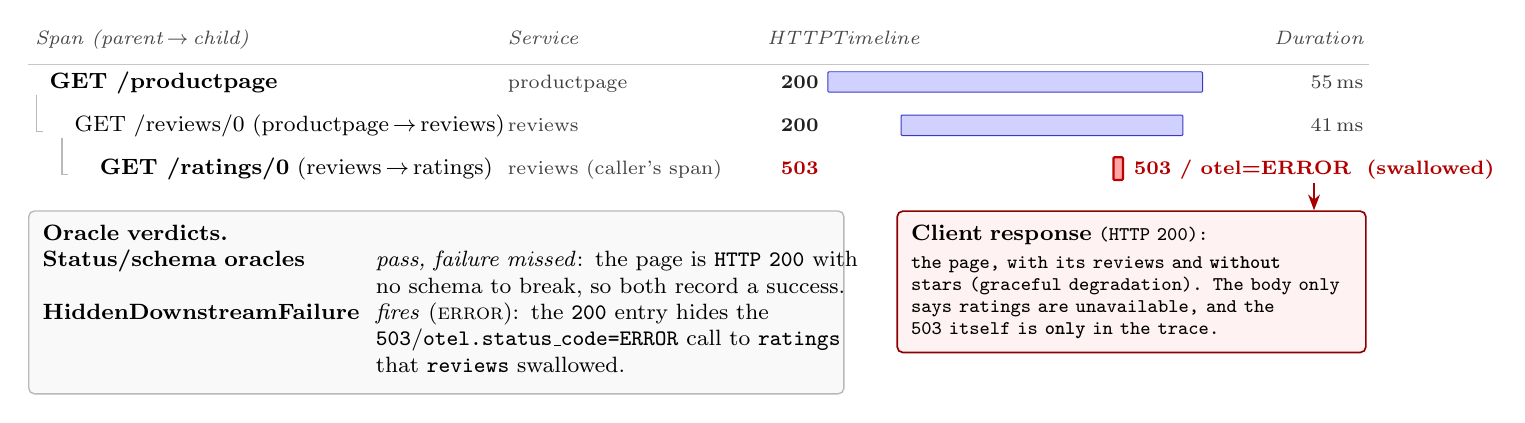
\begin{tikzpicture}[
  font=\footnotesize,
  >={Stealth[length=2mm]},
  % --- Row text styles ---
  spanlbl/.style ={anchor=base west, inner sep=1pt, text depth=0pt},
  svclbl/.style  ={anchor=base west, inner sep=1pt, text depth=0pt,
                   font=\scriptsize, text=gray!50!black},
  statlbl/.style ={anchor=base, inner sep=1pt, text depth=0pt,
                   font=\scriptsize\bfseries, text=gray!25!black},
  staterr/.style ={anchor=base, inner sep=1pt, text depth=0pt,
                   font=\scriptsize\bfseries, text=red!70!black},
  durlbl/.style  ={anchor=base east, inner sep=1pt, text depth=0pt,
                   font=\scriptsize, text=gray!45!black},
  hdrlbl/.style  ={anchor=base west, inner sep=1pt,
                   font=\scriptsize\itshape, text=gray!55!black},
  % --- Bar styles (Gantt segments) ---
  bargw/.style   ={draw=blue!55!gray, fill=blue!18, line width=0.35pt,
                   rounded corners=0.4pt, minimum height=2.6mm,
                   inner sep=0pt, anchor=west},
  barar/.style   ={draw=orange!50!brown, fill=orange!20, line width=0.35pt,
                   rounded corners=0.4pt, minimum height=2.6mm,
                   inner sep=0pt, anchor=west},
  barhi/.style   ={draw=red!75!black, fill=red!35, line width=0.8pt,
                   rounded corners=0.4pt, minimum height=2.9mm,
                   inner sep=0pt, anchor=west},
  % --- Tree connector (left-margin hierarchy) ---
  treeln/.style  ={draw=gray!55, line width=0.4pt},
  % --- Bottom-row boxes ---
  vbox/.style    ={draw=gray!55, line width=0.5pt, rounded corners=2pt,
                   fill=gray!5, align=left, inner sep=5pt,
                   font=\footnotesize, text width=10cm},
  bodybox/.style ={draw=red!55!black, line width=0.6pt, rounded corners=2pt,
                   fill=red!5, align=left, inner sep=5pt,
                   font=\scriptsize\ttfamily, text width=5.6cm}
]

% =============================================================================
% Header row
% =============================================================================
\node[hdrlbl] at (0.00, 0.55) {Span (parent\,$\to$\,child)};
\node[hdrlbl] at (6.00, 0.55) {Service};
\node[hdrlbl, anchor=base] at (9.75, 0.55) {HTTP};
\node[hdrlbl] at (10.10, 0.55)
  {Timeline};
\node[hdrlbl, anchor=base east] at (16.95, 0.55) {Duration};
\draw[gray!45, line width=0.3pt] (-0.05, 0.30) -- (16.98, 0.30);

% =============================================================================
% Span rows (productpage -> reviews -> ratings), real outage trace.
%   timeline bar col   x in [10.10, 14.95]   (10 ms = 0.865 cm)
% =============================================================================

% Row A : GET /productpage  @ productpage   55 ms, 200  (client-facing entry)
\node[spanlbl] at (0.18,  0.00) {\textbf{GET /productpage}};
\node[svclbl]  at (6.00,  0.00) {productpage};
\node[statlbl] at (9.75,  0.00) {200};
\node[bargw, minimum width=4.760cm] at (10.100,  0.08) {};
\node[durlbl]  at (16.95, 0.00) {55\,ms};

% Row B : GET reviews  @ reviews   41 ms, 200  (the reviews server span, starts +10.7 ms; swallows the failure)
\node[spanlbl] at (0.50, -0.55) {GET /reviews/0  (productpage\,$\to$\,reviews)};
\node[svclbl]  at (6.00, -0.55) {reviews};
\node[statlbl] at (9.75, -0.55) {200};
\node[bargw, minimum width=3.580cm] at (11.030, -0.47) {};
\node[durlbl]  at (16.95, -0.55) {41\,ms};

% Row C : GET ratings  @ ratings   0.3 ms, 503 + otel=ERROR  [highlighted: swallowed downstream failure]
\node[spanlbl] at (0.82, -1.10) {\textbf{GET /ratings/0}  (reviews\,$\to$\,ratings)};
\node[svclbl]  at (6.00, -1.10) {reviews (caller's span)};
\node[staterr] at (9.75, -1.10) {503};
\node[barhi, minimum width=0.120cm] at (13.720, -1.02) {};
\node[anchor=base west, font=\scriptsize\bfseries, text=red!70!black, inner sep=1pt]
      (errtag) at (13.95, -1.10) {503 / otel=ERROR \;(swallowed)};

% --- Hierarchical tree connectors in the left margin.
\draw[treeln] (0.06, -0.08) -- (0.06, -0.55) -- (0.14, -0.55);
\draw[treeln] (0.38, -0.63) -- (0.38, -1.10) -- (0.46, -1.10);

% =============================================================================
% Trace Shape Oracle verdict (bottom-left)
% =============================================================================
\node[vbox, anchor=north west] (vrd) at (-0.05, -1.55) {%
\textbf{Oracle verdicts.}\\[2pt]
\begin{tabular}{@{}l@{\hspace{0.7em}}p{6.4cm}@{}}
\textbf{Status/schema oracles} & \emph{pass, failure missed}: the page is \texttt{HTTP 200} with no schema to break, so both record a success. \\
\textbf{HiddenDownstreamFailure} & \emph{fires} (\textsc{error}): the \texttt{200} entry hides the \texttt{503}/\texttt{otel.status\_code=ERROR} call to \texttt{ratings} that \texttt{reviews} swallowed. \\
\end{tabular}};

% =============================================================================
% Client response callout (bottom-right)
% =============================================================================
\node[bodybox, anchor=north east] (body) at (16.95, -1.55) {%
\textnormal{\footnotesize\textbf{Client response}} (HTTP 200):\\[2pt]
the page, with its reviews and \textbf{without}\\
stars (graceful degradation). The body only\\
says ratings are unavailable, and the\\
\texttt{503} itself is \textbf{only} in the trace.};

% --- Arrow: swallowed tag drops to the response callout ---
\draw[->, thick, red!65!black]
     (errtag.south) -- (errtag.south |- body.north);

\end{tikzpicture}
}
  \caption{A trace of \texttt{GET /productpage} on Istio Bookinfo under a \texttt{ratings} outage (checked-in trace, \texttt{details} call not drawn). The page returns \texttt{200} and its body only notes that ratings are unavailable, while the failed call and its \texttt{503} are in the trace alone.}
  \label{fig:trace}
\end{figure*}

% =============================================================================
\section{Motivating Examples}\label{sec:motiv}

Two failures and one generator pitfall motivate MIST. The failures pass any oracle that reads only the status of the client's response, and the pitfall makes a generator report defects that are not there.

Fig.~\ref{fig:trace} shows a trace from Istio Bookinfo under a \texttt{ratings} outage (the service scaled to zero). The entry call \texttt{GET /productpage} returns \texttt{200} because \texttt{reviews} degrades gracefully when \texttt{ratings} is down: the page comes back with its reviews and without stars. The absent \texttt{ratings} emits nothing, so the trace has the call from \texttt{reviews} to \texttt{ratings} as a span recorded on the caller's side with HTTP \texttt{503} and span status \texttt{ERROR} (the \texttt{otel.status\_code} attribute). \texttt{reviews} swallowed the error and answered \texttt{200} anyway. A status oracle records a pass, and a schema oracle has nothing to flag on an HTML page. The body only notes that ratings are unavailable, and the \texttt{503} itself appears only in the trace. We call this a \emph{hidden downstream failure} (MACROHIVE~\cite{Giamattei2022MACROHIVE} calls it a masked failure): a 2xx entry response that masks a server error in a deeper span.

On TrainTicket, the admin route operation \texttt{POST /api/v1/\allowbreak adminrouteservice/\allowbreak adminroute} answers \texttt{HTTP 200} with the body \texttt{\{"status":0,\allowbreak{} "msg":"start or end station not include in stationList.",\allowbreak{} "data":null\}} when it rejects a route. The status class says success and only the body says the request failed. We call this a \emph{soft error}.

The pitfall is fabricated state. Internal endpoints expect state that only earlier calls create, such as an \texttt{orderId} the database knows. A generator that drives them directly must invent that state, and the rejection of an invented value looks like a defect.

% =============================================================================
\section{The MIST Tool}\label{sec:tool}

\begin{figure*}[t]
  \centering
  \resizebox{\textwidth}{!}{% Figure 2 (SANER 2027 order; Figure 1 in the ISSTA version): MIST architecture, three Maven modules.
%   mist-core  : owns the five architectural stages (i)-(v), drawn as one box.
%   mist-cli   : entry mist.jar launcher, JUnit / REST-Assured writer, executor;
%                inputs enter and outputs leave through it.
%   mist-llm   : LLM dispatch and call cache.
% mist-cli and mist-llm each exchange with mist-core over a bidirectional arrow.
% mist-core drives the System Under Test and reads its traces back.
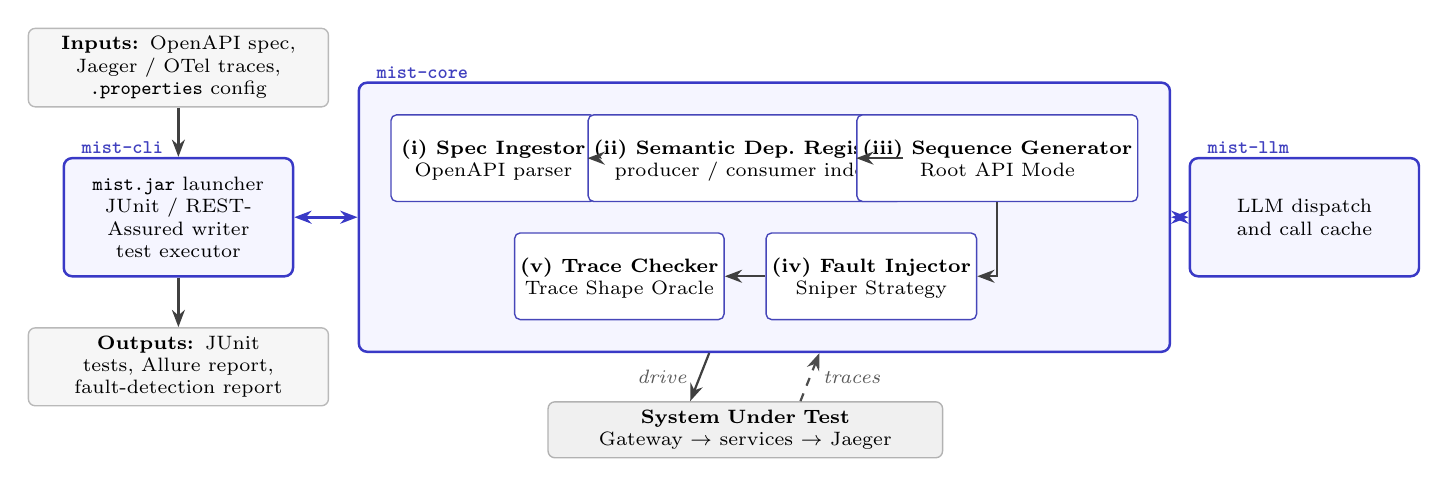
\begin{tikzpicture}[
  font=\small,
  >={Stealth[length=2.2mm]},
  stage/.style  ={draw=blue!45!gray, line width=0.5pt, rounded corners=2pt,
                  fill=white, minimum width=26mm, minimum height=11mm,
                  align=center, inner sep=2pt, text depth=0pt, font=\scriptsize},
  module/.style ={draw=blue!55!gray, line width=0.9pt, rounded corners=3pt,
                  fill=blue!4},
  modbox/.style ={module, align=center, inner sep=3pt, font=\scriptsize,
                  text width=27mm, minimum height=15mm},
  io/.style     ={draw=gray!55, line width=0.5pt, rounded corners=2.5pt,
                  fill=gray!7, align=center, inner sep=3pt, font=\scriptsize,
                  text width=36mm},
  sut/.style    ={draw=gray!60, line width=0.5pt, rounded corners=2.5pt,
                  fill=gray!12, align=center, inner sep=3pt, font=\scriptsize,
                  text width=48mm},
  modlbl/.style ={font=\scriptsize\bfseries\ttfamily, text=blue!50!gray,
                  fill=white, inner sep=1pt, rounded corners=1pt},
  flow/.style   ={->, thick, draw=black!75},
  bidir/.style  ={<->, line width=1.1pt, draw=blue!55!gray},
  trace/.style  ={->, thick, dashed, draw=black!70}
]

% ---- mist-core: the five stages (i)-(v), serpentine flow ----
\node[stage] (ingest)   at (5.0, 0.85)  {\textbf{(i) Spec Ingestor}\\OpenAPI parser};
\node[stage] (registry) at (8.2, 0.85)  {\textbf{(ii) Semantic Dep.\ Registry}\\producer / consumer index};
\node[stage] (gen)      at (11.4, 0.85)  {\textbf{(iii) Sequence Generator}\\Root API Mode};
\node[stage] (mut)      at (9.8, -0.65)  {\textbf{(iv) Fault Injector}\\Sniper Strategy};
\node[stage] (oracle)   at (6.6, -0.65)  {\textbf{(v) Trace Checker}\\Trace Shape Oracle};

\begin{scope}[on background layer]
  \node[module, fit=(ingest)(registry)(gen)(mut)(oracle), inner sep=4mm] (core) {};
\end{scope}
\node[modlbl, anchor=south west] at ([xshift=2mm]core.north west) {mist-core};

% internal flow: i -> ii -> iii (top), down to iv, iv -> v (bottom)
\draw[flow] (ingest)   -- (registry);
\draw[flow] (registry) -- (gen);
\draw[flow] (gen.south) |- (mut.east);
\draw[flow] (mut)      -- (oracle);

% ---- mist-cli (left): inputs/outputs hub ----
\node[modbox] (cli) at (1.0, 0.1)
  {\texttt{mist.jar} launcher\\JUnit / REST-Assured writer\\test executor};
\node[modlbl, anchor=south west] at ([xshift=2mm]cli.north west) {mist-cli};

% ---- mist-llm (right) ----
\node[modbox] (llm) at (15.3, 0.1)
  {LLM dispatch\\and call cache};
\node[modlbl, anchor=south west] at ([xshift=2mm]llm.north west) {mist-llm};

% bidirectional module exchanges
\draw[bidir] (cli.east)  -- (core.west);
\draw[bidir] (core.east) -- (llm.west);

% ---- Inputs (into mist-cli) ----
\node[io] (inputs) at (1.0, 2.0)
  {\textbf{Inputs:} OpenAPI spec, Jaeger / OTel traces, \texttt{.properties} config};
\draw[flow] (inputs) -- (cli);

% ---- Outputs (from mist-cli) ----
\node[io] (out) at (1.0, -1.8)
  {\textbf{Outputs:} JUnit tests, Allure report, fault-detection report};
\draw[flow] (cli) -- (out);

% ---- System Under Test (driven by mist-core, traces flow back) ----
\node[sut] (sutb) at (8.2, -2.6)
  {\textbf{System Under Test}\\Gateway $\to$ services $\to$ Jaeger};
\draw[flow]  ([xshift=-7mm]core.south) -- ([xshift=-7mm]sutb.north)
             node[midway, left=1pt, font=\scriptsize\itshape, text=black!65] {drive};
\draw[trace] ([xshift=7mm]sutb.north) -- ([xshift=7mm]core.south)
             node[midway, right=1pt, font=\scriptsize\itshape, text=black!65] {traces};

\end{tikzpicture}
}
  \caption{MIST's three modules and the five stages of \texttt{mist-core}. The dashed arrow brings each step's trace back from the system under test.}
  \label{fig:arch}
\end{figure*}

\subsection{Architecture}\label{sec:arch}

MIST runs a pipeline of five stages (Fig.~\ref{fig:arch}). Stage (i) parses one OpenAPI document into MIST's configuration. Stage (ii) records, for every identifier-like parameter such as an \texttt{orderId}, which earlier operation and response field produce such a value. This is the producer-consumer inference of RESTler~\cite{Atlidakis2019RESTler}, drawn from the specification, with the captured traces as a fallback. Stage (iii) turns each captured trace into a scenario that keeps its calls in their observed order, merges scenarios linked by a shared value or session, and writes one JUnit~\cite{JUnit4} step per call to be re-issued. Root API Mode (Section~\ref{sec:rootmode}) decides which calls those are. Stage (iv) turns positive tests into negative ones with the Sniper Strategy (Section~\ref{sec:sniper}). A positive test sends requests the system should accept, and a negative test sends requests it should reject. Stage (v) pulls the Jaeger trace after every executed step and checks it against the Trace Shape Oracle's invariants (Section~\ref{sec:traceoracle}).

Take Bookinfo's operation \texttt{GET /api/\allowbreak v1/\allowbreak products/\allowbreak\{id\}/\allowbreak reviews}. Stage (i) reads it from the OpenAPI document. A captured trace holds a client's call to it for product 0, the catalog's only product, and stage (iii) re-issues that call from outside, while \texttt{reviews} still makes its own call to \texttt{ratings}. Stage (iv) derives negative tests that each change only the id, such as the overflow value \texttt{-2147483649}. Stage (v) judges each test by its own new trace. With \texttt{ratings} stopped, the positive test's entry call returns \texttt{200}, but its trace holds the \texttt{503} of the call from \texttt{reviews} to \texttt{ratings}. The oracle reports that call at \textsc{error}, so the positive test fails. The negative test with that overflow value gets \texttt{404} and passes.

MIST has three modules (Fig.~\ref{fig:arch}). \texttt{mist-core} holds the pipeline. \texttt{mist-cli} ships the launcher \texttt{mist.jar}, the writer of JUnit test classes and the test executor. \texttt{mist-llm} calls a language model and caches the answers. When a model is configured, several features call it. Among them are the soft-error classifier (Section~\ref{sec:traceoracle}), a mode in which the model proposes the invalid values for regular-expression and semantic mismatches, and a note the model writes on a step whose trace holds an error. The invariant that flags hidden downstream failures (Section~\ref{sec:traceoracle}) never calls it.

\subsection{Root API Mode}\label{sec:rootmode}

From each captured trace, Root API Mode keeps the one call a client made from outside: the parentless span that remains after skipping the spans of the gateway and service mesh that only route it. MIST calls the same operation from outside and observes the internal services through the trace this call produces. A test can still hold several entry calls, one per captured request, in their observed order. With the mode off, MIST also drives the internal calls directly. With it on, the system creates its own internal state while it serves the entry call, which avoids the generator pitfall of Section~\ref{sec:motiv}.
\subsection{Sniper Strategy}\label{sec:sniper}

Mutating several parameters at once leaves the oracle unable to blame an anomaly on any one of them. An invalid input can also be masked by invalid values in the other calls of the same test. The Sniper Strategy addresses both problems with the classic rule of one invalid condition per test case~\cite{Myers1979ArtOfSoftwareTesting}. In one entry call of a negative test, it sets exactly one parameter, picked round-robin, to an invalid value. The value comes from one of nine categories: type mismatch, regular-expression mismatch, semantic mismatch, overflow, empty input, null input, special characters, boundary violation and enum violation. Each category applies only to the parameter types it fits. Every other parameter, in that call and in the other calls, takes a real value from the captured traces or from an earlier step of the test, so the targeted parameter is the only deliberately invalid input in the test. The exception is a parameter of MIST's configuration for which no earlier response supplies a real value, so MIST invents one.

\subsection{Trace Shape Oracle}\label{sec:traceoracle}

The Trace Shape Oracle evaluates the trace of each executed step against invariants. The central one, the hidden-failure invariant \HDF{}, fires when the entry call returned 2xx while a deeper span server-errored, with an HTTP status of 500 or more or a span status of \texttt{ERROR}. On the product page of Fig.~\ref{fig:trace}, it fires on the call from \texttt{reviews} to \texttt{ratings}. A deeper 4xx alone is benign, because it is usually control flow, such as a lookup miss. The invariant needs no labelled traces, no learned baseline and no model.

A swallowed HTTP 5xx fails a positive test at severity \textsc{error}. A span-status-only error, the gRPC case, raises a \textsc{warn} that is reported without failing the test, because a span status without a 5xx can also mark an internal or tolerated error.

Three further invariants compare a trace with traces from runs known to be good. They flag a missing internal call, a status not seen at that depth before, or a latency above the learned range. They need such traces for each system, and in the runs of Table~\ref{tab:verdicts} they raise nothing.

The soft-error classifier reads response bodies: it classifies the first unseen value of a body's status field (such as \texttt{status:0}) with one language-model call and caches the answer. It then flags any later \texttt{status:0} body without further calls.

\subsection{Using MIST}\label{sec:usage}

A session has three parts. First, the user writes one properties file: the OpenAPI document, the trace sources (a directory of captured traces and a Jaeger URL), the base URL of the system, the authentication settings, and the switches. The switches control Root API Mode, invalid-input categories, invariants and execution.

Second, the user runs \texttt{java -jar mist.jar <file>} on JDK 21. MIST generates, compiles and executes the JUnit classes in the same JVM. Its test client sends a W3C \texttt{traceparent} header with every request, and MIST pulls each step's trace by that header's trace id, or by time window when that lookup finds nothing. It writes three outputs: the classes; Allure~\cite{AllureReport} test results with every step's request, response and trace; and a fault-detection report.

Third, the user reads two reports. In the Allure report, a finding of the hidden-failure invariant names the swallowed span and its status (Fig.~\ref{fig:allure}). The fault-detection report lists the invariant findings and, for a system with planted defects, the tests that triggered each.

By default, MIST turns on Root API Mode, the nine categories, and the invariants for missing calls and unseen statuses, which stay silent until traces of good runs exist. The hidden-failure invariant, the latency invariant and the soft-error classifier are opt-in. The bundled properties files turn the classifier on, and every run of Section~\ref{sec:case} after the TrainTicket benchmark also turns the hidden-failure invariant on.

Adding a system needs the same inputs and no adapter code (examples under \texttt{evaluation/suts/}). For Online Boutique, whose frontend serves HTML, we wrote an OpenAPI document of nine HTTP routes from its route handlers, and MIST generated its configuration from it. Captured page traces and one properties file complete the inputs.

A fresh clone replays the Bookinfo verdict and generates TrainTicket tests without a running system or a model:
\par\noindent\begin{minipage}{\columnwidth}
\begin{lstlisting}[basicstyle=\scriptsize\ttfamily,frame=none]
$ mvn -DskipTests install
$ JAR=mist-cli/target/mist.jar
$ C=mist-cli/src/main/resources/My-Example
$ java -jar $JAR $C/trainticket-demo-noexec.properties
$ D=docs/main-contribution/evidence/bookinfo_html_entry_20261013
$ T=$D/traces/outage_productpage.json
$ java -cp $JAR evaluation/suts/bookinfo/OracleCheck.java \
    $T "GET /productpage"
\end{lstlisting}
\end{minipage}
The \texttt{java -jar} line generates TrainTicket tests offline. The \texttt{OracleCheck} line replays the invariant on a checked-in Bookinfo outage trace and prints the verdict that a status or schema oracle would miss. The repository also holds a harness that repeats the classifier's check against the live model. It needs an API key for the model, and its transcript is checked in.

\begin{figure}[t]
  \centering
  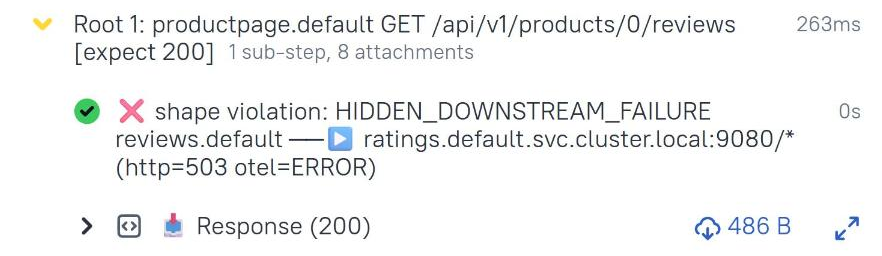
\includegraphics[width=\columnwidth]{figures/allure_finding.png}
  \caption{A failed test in the Allure report (Bookinfo, run of 13 Oct. 2026): the entry call returned \texttt{200}, and the sub-step names the call from \texttt{reviews} to \texttt{ratings} that failed with \texttt{503}.}
  \label{fig:allure}
\end{figure}

% =============================================================================
\section{Case Studies}\label{sec:case}

MIST changes only the requests it sends: the planted defects and the outages below are our experimental setup. We report four systems, each run from its own OpenAPI \mbox{document}, properties file and captured traces. The records behind each result below are in the repository under \texttt{docs/\allowbreak main-contribution/\allowbreak evidence/}. The Sock Shop runs and the outage runs of Bookinfo and Online Boutique below are those of Table~\ref{tab:verdicts}, which adds runs of Bookinfo and Online Boutique without an outage. In every run of Table~\ref{tab:verdicts}, each test sends a distinct request, Root API Mode and the hidden-failure invariant are on, and the model is off. MIST waited ten seconds on Bookinfo and five on Online Boutique, TrainTicket and the logged-in Sock Shop runs before each trace lookup.

We take each operation's call path from the deployment, which the invariant never reads. A test counts as hidden when its entry call answered \texttt{2xx} and either its operation's call path crossed the failed service or the trace it attached holds a failed span. A hidden test counts as missed when the invariant passed it. A flag counts as on path when the span the invariant listed lies on the operation's call path and carries a \texttt{5xx} or an error status in the trace the test attached.

In the three outage runs, every 2xx test of an operation that calls the stopped service was flagged on the call to it. All 665 flags over 3,204 tests were on path, and the invariant fired on every hidden test.

\begin{table}[t]
\centering
\caption{The hidden-failure invariant's verdict on every test of one run per system state, with the language model off ($\dagger$: at \textsc{warn}). Section~\ref{sec:case} defines the columns.}
\label{tab:verdicts}
\scriptsize\setlength{\tabcolsep}{2.5pt}
\begin{tabular}{@{}llrrrrr@{}}
\toprule
\textbf{System} & \textbf{State} & \textbf{Tests} & \textbf{Hidden} & \textbf{Fired} & \textbf{On path} & \textbf{Missed} \\
\midrule
Bookinfo        & no outage               &  70 &   0 &   0 &   0 & 0 \\
Bookinfo        & \texttt{ratings} down   &  70 &   1 &   1 &   1 & 0 \\
Online Boutique & no outage               & 543 &   0 &   0 &   0 & 0 \\
Online Boutique & \texttt{adservice} down & 543 &  10 &  10$^{\dagger}$ &  10 & 0 \\
Sock Shop       & no login, no outage     & 511 & 354 & 354 & 354 & 0 \\
Sock Shop       & login, no outage        & 511 &  72 &  72 &  72 & 0 \\
Sock Shop       & login, \texttt{catalogue} down & 511 & 228 & 228 & 228 & 0 \\
TrainTicket     & no outage, 8 services   & 445 &   0 &   0 &   0 & 0 \\
\bottomrule
\end{tabular}
\end{table}

\subsection{TrainTicket: Generation at Scale}

For a benchmark run, we planted ten input-validation defects in TrainTicket's services. A list names the planted defects, the planted code returns a defect's name in its response, and MIST records which tests triggered each one. On that build, MIST generated and executed 15,036 tests in about 6.5 hours, and they triggered all ten defects. This is a generation and scale result: the planted code's own report, not the trace oracle, identifies each triggered defect. A run on eight services of the planted-defect build (Table~\ref{tab:verdicts}) raised no flag: the planted defects answer \texttt{400}, not a 2xx. The planted defects play the part of mutants in mutation testing~\cite{Jia2011MutationSurvey}: seeded faults whose triggering measures the generated inputs.

\subsection{Istio Bookinfo: The Hidden 503}

The walkthrough of Section~\ref{sec:arch} is the outage run of Table~\ref{tab:verdicts}, with \texttt{ratings} scaled to zero, and none of the operation's negative tests got a 2xx. In a separate run on the page of Fig.~\ref{fig:trace}, MIST generated one test from a captured trace, and the invariant fired at \textsc{error} on the same swallowed call. Run against the same outage, EvoMaster 6.2.0~\cite{Arcuri2019EvoMasterTOSEM} (black-box) and Schemathesis 4.23.0~\cite{HatfieldDodds2022Schemathesis} pass the page's \texttt{200} response, which breaks no schema.

\subsection{Online Boutique: The Same Failure over gRPC}

With \texttt{adservice} scaled to zero, the positive tests of the home page and all nine product pages each got \texttt{200}. The invariant raised \textsc{warn} on the swallowed call from \texttt{frontend} to \texttt{adservice}, whose gRPC status is 14 (unavailable) while its HTTP status attribute reads a misleading \texttt{200}. The home page answers a clean \texttt{200} with no error text, so only the trace exposes the failure.

\subsection{Sock Shop: Generated Requests and an Outage}

On Sock Shop with no outage, all 352 tests of \texttt{POST /addresses} and \texttt{POST /cards}, generated as positive and negative alike, sent one request each without a login session and got \texttt{200} from the front-end with an error body. Behind each, the \texttt{user} service had failed with \texttt{500} or a sidecar with \texttt{503}, and the invariant fired at \textsc{error} on each. On most of them the service cannot parse the customer id, which is absent without a login session. On two GET tests whose generated \texttt{size} value overflowed, the invariant fired on a \texttt{503} behind a \texttt{200}. In a logged-in run, the invariant flagged no positive test, and its 72 flags came from invalid inputs, such as a JSON value of the wrong type, on which the called service failed. In a second logged-in run with \texttt{catalogue} stopped, the front-end answered all 159 catalogue reads with \texttt{200} and the body \texttt{no healthy upstream}, and the invariant flagged each on the call to \texttt{catalogue}. Its other 69 flags there came from invalid inputs, as in the first logged-in run. A status oracle sees no server error in any of these responses.
% =============================================================================
\section{Related Work}\label{sec:rw}

EvoMaster~\cite{Arcuri2019EvoMasterTOSEM}, RESTler~\cite{Atlidakis2019RESTler}, RESTest~\cite{MartinLopez2021RESTest}, RestTestGen~\cite{Corradini2022RestTestGen}, Schemathesis~\cite{HatfieldDodds2022Schemathesis} and Morest~\cite{Liu2022MoRest} generate requests from the OpenAPI document, and ARAT-RL~\cite{Kim2023ARATRL} and AutoRestTest~\cite{Stennett2025AutoRestTest,Kim2025AutoRestTestSPDG} add reinforcement learning. All of them judge a response mainly by its status class and schema. A soft error whose body keeps its usual shape passes both. So does a hidden downstream failure whenever the degraded response breaks no schema, as on Bookinfo's product page and on Online Boutique (Section~\ref{sec:case}).

AGORA~\cite{Alonso2023AGORA} and its journal extension~\cite{Alonso2026TOSEMOracles} infer invariants over responses from API executions, and SATORI~\cite{Alonso2025SATORI} infers response-field oracles statically from the specification. LogiAgent~\cite{Zhang2025LogiAgent} has a language model read each response body, and RESTifAI~\cite{Kogler2025RESTifAI} derives expected 2xx and 4xx outcomes from generated happy paths. All of them read the response or the specification and never the cross-service trace, so a swallowed failure behind a clean body escapes them.

MACROHIVE~\cite{Giamattei2022MACROHIVE} exposes masked failures through a proxy deployed beside every service, while MIST reads them from the trace the services export. Tracetest~\cite{Tracetest}, an industrial trace-assertion product, asserts over spans but needs a person to write each assertion, and it neither generates tests nor mines traces. TraceRCA~\cite{Li2021TraceRCA} and Nezha~\cite{Yu2023Nezha} explain an incident from production traces after the fact, whereas MIST uses the trace during testing, as an oracle on a generated test. To our knowledge, MIST is the first open-source REST API test generator that uses a system's own trace both as generation input and as functional oracle.

% =============================================================================
\section{Limitations and Conclusion}\label{sec:concl}

MIST sees only what the system exports: uninstrumented services are invisible, and a swallowed failure that leaves no errored span is missed. The hidden-failure invariant encodes a policy: the same trace can be intended graceful degradation, and the invariant counts every server-errored span, retried or not. In live checks against the model, the classifier catches TrainTicket's \texttt{status:0} body but misses an error body like the one Sock Shop's front-end returned, so soft-error detection stays the lower-assurance part of the oracle.

MIST turns the OpenAPI document and the traces a microservice system already exports into cross-service tests, and checks each run against the trace it retrieves for that run. In that trace, the hidden-failure invariant flags the failed call that the status oracle passes. The source code is at \url{https://github.com/miaoti/MIST/} under LGPL-3.0. A repository snapshot is archived at \url{https://doi.org/10.5281/zenodo.23359365}.
\bibliographystyle{IEEEtran}
\bibliography{refs}

\end{document}
